\chapter{What's ungrammatical}


\begin{itemize}
    \item There is a common way to say something, a construction that pairs meaning with form.
    \item When something fails to follow this, we assume some new function.
    \item If no such function can be found, it feels ungrammatical.
\end{itemize}

%It's easier to say what is not grammatical than to say what is. Things may be ungrammatical in a relative or absolute sense, relative to a particular language, or simply not possible in human language \citep{Leivada2020} eg. \textit{The doctor the nurse the hospital had hired met John.} (Frazier 1985)


\section{\textit{I go there yesterday}}

\textit{I go there yesterday} sets up a clash between the present tense of the verb, which signals non-past time, and the past-time meaning of the modifier \textit{yesterday}.

\ea\label{ex:go-yesterday-clash}
    \begin{dialogue}
        \speak{Son} \phantom{..*}\textit{Hi, Mom.}
        \speak{Mom} \phantom{*}\textit{Hi, Honey! Where were you?}
        \speak{Son} \phantom{..*}\textit{The new bookstore.}
        \speak{Mom} *\textit{Oh, \myuline{I go there yesterday}.}
    \end{dialogue}
\z

Our default assumption is that Mom is not just messing up here. We attribute intentionality her choice of present-tense \textit{go} + \textit{yesterday}. Assuming a clash like this is intended, though, sends Son (and us) on a search for a reason, a quest that hits a dead end, as no justification presents itself. And so we register the underlined clause as ungrammatical.

%And this cost us. Our pupils dilated reflecting the mental effort to resolve the clash. Our heart rate variability dropped.

But could \textit{I go there yesterday} ever be grammatical?

\ea\label{ex:go-yesterday-effective}
    \begin{dialogue}
        \speak{Son} \phantom{..*}\textit{Hi, Mom.}
        \speak{Mom} \phantom{*}\textit{Hi, Honey! Where were you?}
        \speak{Son} \phantom{..*}\textit{The new bookstore.}
        \speak{Mom} \phantom{*}\textit{Oh, you won't believe this. So, \myuline{I go there yesterday}, and\dots}
    \end{dialogue}
\z

In this iteration, Mom offers a vital interpretive key: she is initiating a story. The present-tense form \textit{go}, clashing with the past-oriented \textit{yesterday}, is now reconceptualized as a story-telling technique. We're able to see an -- likely \textit{the} -- intended purpose behind it: a sense of immediacy and involvement in the storytelling, making what was sharply ungrammatical in (\ref{ex:go-yesterday-clash}) indisputably grammatical in (\ref{ex:go-yesterday-effective}).

\begin{center}
    -- --
\end{center}

As Old French became Middle French in the fourteenth century and gradually evolved into Modern French, the present perfect was becoming a past tense in a striking example of various pressures and motivations allowing the ungrammatical to become grammatical.

Until the fourteenth century, French and English had matching simple-past and present-perfect tenses. The simple past looked like this: \textit{Je \uline{changai} mon avis} `I changed my mind', and the present perfect like this: \textit{J'\uline{ai changé} mon avis.} `I have changed my mind'. Though these mean basically the same thing, \textit{changai} `changed' is a past tense while the \textit{ai} of \textit{J'\uline{ai changé}} is the present `have'. That means \textit{J'\uline{ai changé}} is a present tense, albeit a retrospective one. Like the English present perfect, it's anchored in the now but encompasses things past. This makes it very compatible with a word like \textit{recently}, which covers the present and not-too-distant past.

A word like \textit{hier} `yesterday', though, whose meaning is completely separated from the here and now sets up a clash. In Old French, *\textit{J'\uline{ai} changé mon avis \uline{hier}} meant both present (\textit{ai}) and not present (\textit{hier}), making it as ungrammatical as *\textit{I have changed my mind yesterday} in English.

%The `present' meaning of the present perfect can also be seen in discussing event sequencing. Using the past tense, we might say, \textit{He left, and then she arrived,}. But employing the present perfect in similar contexts *\textit{He has left, and then she has arrived} introduces a clash. It suggests his departure is both connected to the present and yet set off from it by her arrival.

To say that the Old-French present perfect turned into a past tense, then, is to say that it lost that `present' meaning, becoming fully compatible with a word like \textit{hier} `yesterday'. In Modern French it's perfectly grammatical to say \textit{J'ai changé mon avis \uline{hier}} because it now means `I changed my mind yesterday,' with no taint of the present. In short, what was the present perfect became the \textsc{passé composé} `the compound past tense'.

Although the meaning of \textit{j'ai changé} has changed, the form really hasn't. It still includes an auxiliary verb, usually \textit{avoir} `have' in its present-tense form, along with the past participle of the verb to be put into the past tense, here \textit{changer} `change'. The full set of forms is shown in Table \ref{tab:have-changed-conjugation}.

\begin{table}[ht]
\centering 
\caption{Formation of the Passé Composé in Modern French}
\label{tab:have-changed-conjugation}
\begin{tabular}{llll}
\toprule
\textbf{Subject} & \textbf{\textit{Avoir}} & \textit{\textbf{Changer}} & \textbf{Translation} \\
\midrule
\textit{j'} & \textit{ai} & \multirow{6}{*}{\raisebox{60pt}{\rdelim\}{6}{10pt}[{}]}\raisebox{26pt}{\textit{changé}}} & `I have changed' \\
\textit{tu}      & \textit{as}  &      & `You have changed' \\
\textit{il/elle} & \textit{a} &    & `He/She has changed' \\
\textit{nous}    & \textit{avons} &    & `We have changed' \\
\textit{vous}    & \textit{avez} &     & `You have changed' \\
\textit{ils/elles} & \textit{ont} &    & `They have changed' \\
\bottomrule
\end{tabular}
\end{table}


\bigskip


There is no simple semantic or syntactic explanation for how this set of verb forms changed its meaning. But when social and phonological factors are accounted for, a potential story begins to emerge.

In Old French, as in its ancestor Latin, stress was typically placed on the penultimate syllable. Over centuries, this resulted in an erosion of the final syllable. For example, Latin \textit{fundaMENtum} became Old French \textit{fondeMENT}, preserving only the $\langle$t$\rangle$ of the last syllable. Even that has been lost in Modern French pronunciation /fɔ̃d.mɑ̃/, though the fossilized spelling remains. This kind of ``Matthew effect''\footnote{From the Gospel of Matthew 25:29, ``For to everyone who has, more will be given...but from the one who has not, even what he has will be taken away.''} where unstressed elements fade away is pervasive and a common driver of change across languages.

Erosion at the end of words is a problem for Latinate languages because that's where the verb conjugations are, and there are a lot of verb conjugations. The simple past tense's troubles start here. Table \ref{table:past_tense_conjugation} shows the robust Old French simple past verb endings and their diminished state in Modern French. 

\begin{table}[ht]
\centering
\begin{tabular}{lll}
\hline
\textbf{Person} & \textbf{Old Fr. (IPA)} & \textbf{Modern Fr. (IPA)} \\
\hline
1st Singular & /naviˈʒai/ & /na.vi.ʒe/ \\
2nd Singular  & /naviˈʒas/ & /na.vi.ʒa/ \\
3rd Singular  & /naviˈʒa/ & /na.vi.ʒa/ \\
1st Plural &  /naviˈʒames/ & /na.vi.ʒɑ̃/ \\
2nd Plural &  /naviˈʒastes/ & /na.vi.ʒat/ \\
3rd Plural &  /naviˈʒaʀənt/ & /na.vi.ʒɛʀ/ \\
\hline
\end{tabular}
\caption{Simple Past Tense Conjugation in Latin, Old French, and Modern French}
\label{table:past_tense_conjugation}
\end{table}

These sound shifts were influenced by various factors. One might have been the social life of teen girls, a demographic that often plays a significant role in accelerating and popularizing linguistic change \citep{labov2001}. Their desire to express their unique identities, their experimentation with language, and their influence within tight-knit social circles often make them drivers of linguistic innovation. Imagine a group of girls subtly tweaking the established stress patterns, perhaps for emphasis within their conversations or simply as a playful new way of speaking. These variations may have caught on within their circle, eventually spreading more broadly.

Whatever the vector, stress shifted, and the waning syllables lost their final consonants like so many autumn leaves. Not in writing, but in speech. Because Old French relied on verb endings to distinguish between, for example, first-person singular and third-person plural within a given tense, not to mention distinguishing among tenses, things got complicated. Pronouns, previously optional as in Modern Italian or Spanish, began to gain importance. 

For Old French, words were generally pronounced as they were spelled. The Old French pronunciations in the table are somewhat speculative, but they're reasonable approximations for the verb \textit{aimer} `love'. This clearly shows that the Old French conjugations are much more distinct than the Modern ones. 

\begin{table}[h]
\centering
\begin{tabular}{lll}
\hline
\textbf{Person}          & \textbf{Old French} & \textbf{Modern French} \\ \hline
1st Singular             & \textit{aim} /aim/   & \textit{j'aime} /ʒɛm/           \\
2nd Singular             & \textit{aimes} /aiməs/ & \textit{tu aimes} /ty ɛm/    \\
3rd Singular             & \textit{aime} /aimə/ & \textit{elle aime} /ɛl ɛm/ \\
1st Plural               & \textit{aimons} /aimɔ̃s/ & \textit{nous aimons} /nu zɛ.mɔ̃/ \\
2nd Plural               & \textit{aimez} /aiməz/ & \textit{vous aimez} /vu zɛ.me/ \\
3rd Plural               & \textit{aiment} /aimənt/ & \textit{ils aiment} /il zɛm/ \\ \hline
\end{tabular}
\caption{Comparative Verb Conjugations in Old French and Modern French with IPA Transcriptions}
\end{table}

As a result, many elements of the simple past began to sound very much alike. Luckily, the irregular nature of the auxiliary verbs for the present perfect (before it became reconceptualized as the passé composé), meant that they were far less subject to this phonemic erosion, and so far less subject to conjugational confusion.

\begin{table}[h]
\centering
\begin{tabular}{lll}
\hline
\textbf{Person} & \textbf{Passé Composé} & \textbf{IPA} \\
\hline
\textit{j'} & \textit{ai aimé} &/e ɛ.me/ \\
\textit{tu} & as aimé &/a ɛ.me/ \\
\textit{il}/\textit{elle} & \textit{a aimé } & /a ɛ.me/ \\
\textit{nous} & \textit{avons aimé} & /a.vɔ̃ ɛ.me/ \\
\textit{vous} & \textit{avez aimé} & /a.ve ɛ.me/ \\
\textit{ils}/\textit{elles} & \textit{ont aimé} & /ɔ̃ ɛ.me/ \\
\hline
\end{tabular}
\caption{Passé Composé Conjugation of \textit{aimer} with IPA Transcriptions}
\end{table}

Since the passé simple and the present perfect could generally be used to refer to the same events, as long as a specific time word like \textit{hier} `yesterday' wasn't used, people started to avoid the more phonologically ambiguous passé simple. If that meant being vague about when something had happened, so be it.

Though this series of changes took roughly 300 years in Paris, they spread much more slowly in the surrounding areas, the result being that the use of the passé simple began to take on a whiff of provincialism, at least in certain uses. Once this had happened, the pressure for Parisians to avoid it was enough to overcome the sense of incompatibility between present nature of the form and the past-nature of the meaning. For them, it had become the passé composé.

\begin{center}
    -- --
\end{center}

We can see just the type of problems that verb-form ambiguity can cause in the famous sentence -- at least relatively famous among linguists -- \textit{The horse raced past the barn fell.} If you've never encountered it before, you likely judged it to be ungrammatical. But I have not starred it because it only gives the illusion of ungrammaticality, an illusion produced by the overlap between the past tense and the past participle, both of which are \textit{raced}.

Past-tense forms are generally more common than past participles, and this is particularly true directly after a noun; the past participle usually follows an auxiliary such as \textit{be} or \textit{have}, as in \textit{the horse \uline{was} raced}. And so we are tricked into believing that \textit{raced} is the past-tense form. But there is a structure in which the participle doesn't need an auxiliary: a post-head modifier, as in, \textit{the horse \uline{seen} on the hill}. Because \textit{see} distinguishes \textit{saw} from \textit{seen} the illusion collapses. In case it's still not clear, the original sentence was \textit{the horse \op which was\cp~raced past the barn fell}.

Despite this occasional overlap between the past tense and past participle in English, our present perfect has not become a past tense. A true past tense, like the passé composé or the simple past in English (again the ``preterite''), means `completed before now'. The English perfect, though, means `looking back from a point', and the \textit{present} perfect establishes that point as `now'. We can often freely choose between the two for any given past even: \textit{I've seen her} or \textit{I saw her}, but *\textit{I've seen her yesterday} is still impossible. The `past-time' meaning of that explicit \textit{yesterday} clashes with the `present-time' meaning of present-tense \textit{have}, and this kind of meaning clash gives rise to feelings of ungrammaticality.

This leads to the question of why we don't we get the same ungrammatical feeling when the paradox is introduced by word choice rather than word forms, as discussed in Section \ref{sec:model-of-grammaticality}. Statements such as \textit{the water was so dry} or \textit{it was too light to pick up}, provoke curiosity rather than discomfort.

Perhaps, lexical choices like this open up many possible interpretations, such as metaphor, exaggeration, and humour, and so we assume that the paradox was intended. The use of the perfect with a past-time reference like \textit{yesterday}, though doesn't suggest such a purpose, and so immediately registers as a grammatical error.

Consider *\textit{I have two cat.} The intended sentence could be \textit{I have one cat} (wrong word) or \textit{I have two cats} (wrong word form), but my guess is that no editor would change \textit{two} to \textit{one}; they would assume the error is in the grammar. Similarly, \textit{I've seen it yesterday} could be \textit{I've seen it recently} (wrong word) or \textit{I saw it yesterday} (wrong tense). Again, I assume that most editors would blame the tense.

In agreement errors like \textit{a group of students are coming}, we assume that the verb form is incorrect rather than that \textit{group} should be \textit{number} or \textit{majority}. In an example like \textit{give the form from Sarah}, lacking context, we set aside the possibility that the lexical word \textit{give} should have been \textit{get} and assume that the ``grammatical word'' \textit{from} should be \textit{to}.

In part, this may be because the degrees of freedom are almost always much smaller with grammar than with lexis. To make this concrete, consider that, across the world's language, the system of number may mark plurality as it does in English -- singularity being unmarked -- or duality and plurality, as in Arabic. A very few, such as Wamesa, mark triality on pronouns. There are a few other ways, such as marking paucality (the state of being few in number), but this mostly exhausts the possibilities for marking grammatical number, apart from not marking number at all. Now consider tallying the possible nouns to which any system of number applies number. The number will be thousands of times greater.

Think of language as a set of Lego blocks. You have a limited number of shapes, and they can only connect in specific ways -- the grammar. If something doesn't fit, you would default to shifting, turning, or trying to connect it in one of those ways rather than assuming you've got the wrong piece. You'd assume you made a placement or ``grammar'' mistake rather than a selection or ``lexical'' mistake. This reflex is born of an understanding that the grammar rules, much like the physical constraints of Lego, are relatively inflexible. A block misplaced by a few degrees or millimetres simply won't connect. But as long as you've got the angle and position right, you've got a lot of latitude about which blocks you use.

This balance isn't inevitable. In constructing an Ikea desk, the ``vocabulary'' of pieces is roughly as constrained as the ``syntax'' of combinations. So, if something's wrong, you might as well guess you've got the wrong piece as that you've put it together the wrong way. Languages, though, are much more like Lego sets than Ikea kits, at least in this regard.

Another way to look at the question of why we default to assuming ungrammaticality is caused by grammar, not words, is simply to ask how likely any given sentence is. Back in 1957, Chomsky attempted to illustrate that answering such a question is simply an impossibility with the famous pair of ``sentences'' in (\ref{ex:colorless-green-ideas}).

\ea \label{ex:colorless-green-ideas}
    \ea[]{\textit{Colorless green ideas sleep furiously.}}
    \ex[]{\textit{Furiously sleep ideas green colorless.}}
    \z
\z

At the time, he asserted without proof that ``in any statistical model for grammaticalness, these sentences will be ruled out on identical grounds as equally `remote' from English'' \citep[15]{Chomsky1957}. Not so!

Most people find (\ref{ex:colorless-green-ideas}a) to be nonsensical but perfectly grammatical. They realize that the words don't add up to anything they could really make sense of, but that other words might, \textit{colorful green leaves rustle gently}, for instance. Consider, though, that for most people at most times, many sentences seem nonsensical: Werner Heisenber's observation that ``the more precisely the position [of an electron] is determined, the more imprecisely will the impulse be known, and vice-versa'' \citep[5]{Heisenberg1927}, or Martin Heidegger's claim that ``the most thought-provoking thing in our thought-provoking time is that we are still not thinking'' \citep{Heidegger1993}, or  Friedrich Nietzsche's aphorism, ``when you stare into the abyss, the abyss stares back at you,'' \citep{NietzscheBeyondGoodAndEvil}, or  Simone de Beauvoir's thought that ``one is not born, but rather becomes, a woman'' \citep{DeBeauvoir1949}. Indeed much of what has been said throughout human history might seem meaningless to most of us. These examples illustrate that we're quite familiar with words being put together to mean things we haven't thought or find difficult to think, but that could, with effort, be rendered sensible. And so, though any one of these confounding strings is highly unlikely in itself, the experience of encountering such unexpected collections of words arranged expectedly (or so it would seem) is just a commonplace, not an aberration as Chomsky claimed.

What is truly remote from our experience is seeing strings like (\ref{ex:colorless-green-ideas}b). \citet{Pereira2000} demonstrates this with a simple bigram model. Imagine language as a network of pathways between pairs of words (bigrams). Some are well-worn superhighways between words that often occur together (\textit{and the}), others overgrown trails between words that almost never co-occur (\textit{my the}). Roughly speaking, Pereira looks at likelihood as the total traffic between any two points. Sentences with the most traffic over the shortest distances are more likely in this model. \textit{Colorless green ideas sleep furiously} doesn't take the main streets, but it uses established routes -- people actually do talk about \textit{green ideas}, though \textit{green} means `environmental' here. Meanwhile, \textit{Furiously sleep ideas green colorless} strikes out on its own, forging new paths at each turn. Under this bigram model, the apparently grammatical but meaningless (a) is not just more likely but roughly 200,000 times more likely than the word salad that is (b) \citep[7]{Pereira2000}.

Returning, though, to the difference between lexical meaning and grammatical meaning, it's clear that the words in Chomsky's sentence do not make semantic sense, but the grammar is fully coherent. It's meanings all work.

There is a subject, meaning that the clause is about something -- it has a topic. It also says there's an agent available to perform the action denoted in the predicate. And the subject is an NP, which is conventional.

The noun phrase (NP) has two adjective phrase (AdjP) modifiers, attributing properties from the lexical adjective heads to the head noun. The absence of a determiner means that the NP is indefinite, and nothing in the sentence contradicts this interpretation. The NP is plural, as marked by the morphology of ideas. This plurality aligns with the systems of determiners, quantification, and definiteness, all conveying coherent meanings. Even the order of adjectives conforms to standard expectations: a general property adjective (\textit{colorless}) followed by a color adjective (\textit{green}) attributed properties to the entity \textit{ideas}.

The verb phrase (VP) exhibits similar coherence in its grammatical meaning. Placed after the subject, the VP indicates that the subject performs the action denoted by the verb. Specifically, \textit{sleep} requires an Agent role, and the subject NP fulfills this by actively engaging in the action. The present-tense verb form suggests that this situation is a general one, not a particular past or future action, which aligns well with the indefinite nature of the subject.

The verb \textit{sleep} requires a subject, and the grammatical relationship -- that the referent of the subject NP performs the action -- is clear and unviolated. The adverb \textit{furiously}, positioned at the end of the VP, attributes a manner to the action, irrespective of whether sleeping can logically be done furiously. The verb agrees with its plural subject, maintaining grammatical agreement. Crucially, although we might question the plausibility of ideas sleeping (especially furiously), this does not violate the grammatical meaning of predication -- that is, the action denoted by the verb is attributed to or performed by the subject's referent. The tense marking is appropriate, the word order adheres to English syntax, and all grammatical subsystems operate without contradiction. The sentence's oddness arises entirely from conflicting lexical meanings, not from any failure in grammatical meaning conveyance.

In short, we have sound justifications for our intuition that some sentences are ungrammatical while others are just puzzling, and that, to fix an ungrammatical string such as \textit{two cat}, it makes sense to fix the grammar rather than the choice of words. 

\bigskip

Another linguistic realm where we encounter the unusual without it registering as ungrammatical is in pronunciation and accent. If one hears talk of a ``bi-O-pic'' about Robert Oppenheimer, one assumes the fault is in the stress pattern (BI-o-pic) and not the choice of words (\textit{myopic}). Again, hearing ``bi-O-pic'' could lead to a moment of confusion, but never a feeling of ungrammaticality.

In this example, the interpretation is constrained by meaning (it's about Oppenheimer) and syntax (\textit{biopic} is a noun, and \textit{myopic} isn't), and we can even reason our way towards an explanation about how the speaker had perhaps only seen \textit{biopic} in print and guessed -- incorrectly -- about an analog with the pronunciation of the similarly spelled \textit{myopic}. But even so, we know that pronunciation is highly variable, or at least we are accustomed to the fact.

It's plain that the vowel in a British \textit{can't} is quite unlike a Canadian \textit{can't}. But what we may not be so aware of is that our own individual vowels have a certain amount of variation. The /æ/ in a Canadian \textit{can't} is realized slightly differently than the one in \textit{hat} which differs again from that in \textit{bag}. Although we mentally classify each as /æ/, there are measurable differences. In fact, your own /æ/ in \textit{hat} differs slightly each time you say the word, perhaps because you're a little more tired, or a little more thirsty, or speaking a little more loudly, or for any of hundreds of other reasons.

An overly simplistic view of this is to liken our perceptual categories to watersheds. The rain that falls in the broad Columbia-River watershed in British Columbia flows into that river, and that which falls on the neighbouring Fraser-River watershed into the Fraser. Similarly, vowels falling anywhere within one perceptual range ``flow down'' into /æ/, while those with sufficiently different frequencies will flow down into the neighbouring /e/. Those perceptual ranges are quite broad, varying by hundreds of hertz or more. And just as minor variations in where the rain falls don't change the broader classification into Columbia or Fraser-River watersheds,  minute variations in how we pronounce a phoneme don't alter our classification of that particular sound.

Here's where the analogy breaks down though: rain that falls into one watershed never flows out of it into the neighbouring river, but phonemes are far more fickle. There's actually a good deal of overlap between some vowel sounds, as illustrated in Figure \ref{fig:vowel-distribution-illustration}. The way a sound is perceived depends a good deal on the surrounding context and what we're expecting. And just as we can coerce certain constructions into being grammatical we can coerce sounds into being perceived as this or that phoneme. 

%Should I include a discussion to introduce the McGurk effect?

\begin{figure}
    \centering
    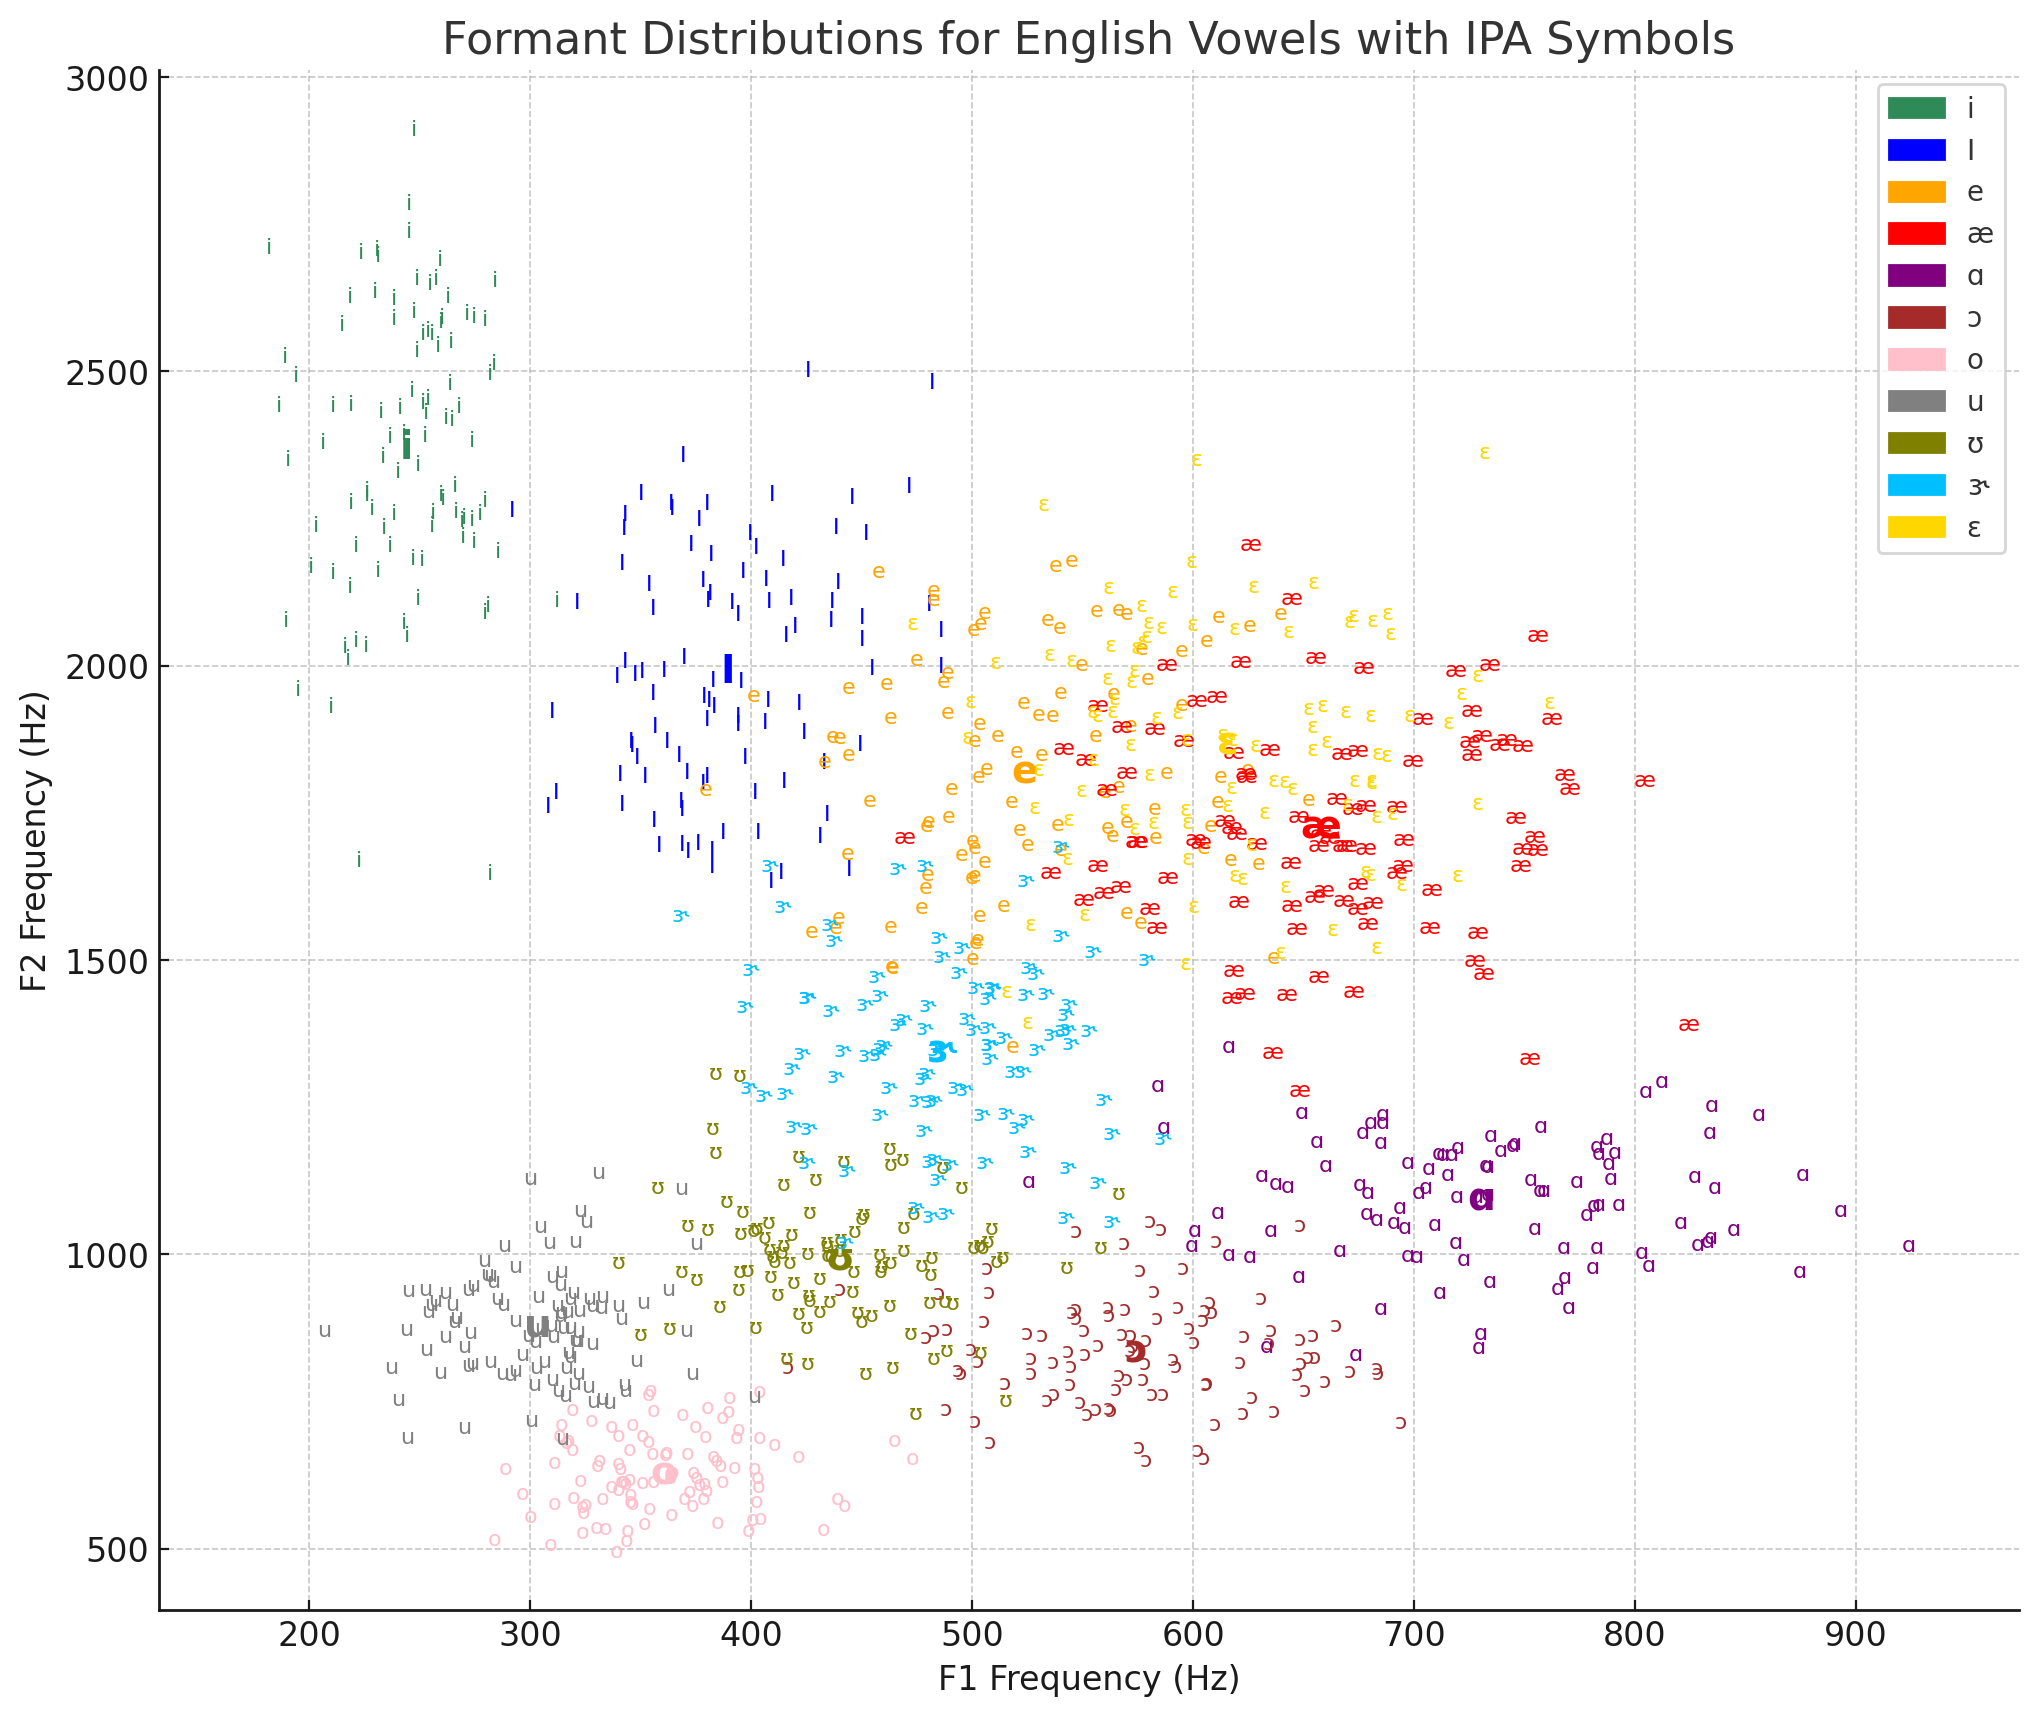
\includegraphics[width=0.8\textwidth]{figures/sampleVowels.png}
    \caption{Simulated overlapping distributions of English vowels. Distributions are illustrative and not based on empirical data.}
    \label{fig:vowel-distribution-illustration}
\end{figure}

Another reason that a form-meaning clash is unlikely at the phonemic level is because, for the most part, phonemes don't mean. Despite claims throughout history for an iconic connection, such as those of Cratylus in Plato's \textit{Cratylus}, words don't have a natural correctness; that is, they are arbitrarily, not inherently, linked to the concepts they denote.

Cratylus argues that every word is not just a random label but is crafted with an understanding of what it denotes. This implies that a kind of philosophical insight into the nature of things is embedded in the very language we use. For example, according to his perspective, the phoneme /s/ in \textit{sun} could be seen as naturally indicative of the qualities or essence of the sun itself. He might argue that /s/ captures an aspect of the sun's essence, perhaps its hissing, radiant heat, or the sharpness of its light. This phoneme, under Cratylus's view, is iconic. It's linked to the concept of the sun by some inherent resemblance between the two.

But this can't work. If someone like me who knows no Persian encounters a word like \textit{sib}, I have no way of working out its meaning from the pronunciation /siːb/. The presence of the /s/ is entirely unhelpful, let alone reliable in signalling some kind of hissing, radiant heat, or sharpness of light. It is simply impossible to deduce from phonology alone that \textit{sib} means `apple' in Persian but `goat' in Zoogocho Zapotec. And if I thought that its meaning might be similar to the meaning of /ziːb/ or /sɪb/ or or /ziːp/ because they sound very similar, well, I would just be wrong. That's not how it works. The association between a word's meaning and its pronunciation is mostly arbitrary.

I say ``mostly'' arbitrary because some phonemes really do appear to be iconic. In 2022, \citet{Winter2022} published a massive, cross-cultural, multi-language set of four studies of the textural iconicity of a trilled /r/. If asked about the texture that phoneme evokes, what would you guess?

Their studies involved participants from diverse linguistic backgrounds who, despite their varied languages, consistently linked the trilled /r/ with a sense of roughness or vibration, akin to the texture one feels when touching a coarse surface.  This convergence across cultures indicates that our sensory experiences can shape and be mirrored in our linguistic practices. But don't forget that trilled /r/ was the first such pattern shown to apply across a wide range of the world's languages, as well as to various words within those languages. The lack of other documented cases suggest that it is special. Even so, its iconicity doesn't apply consistently (consider \textit{creamy}, \textit{murmur}, and \textit{serene}), and its applicability is limited to sensory words.


What it all comes down to is that phonetic variability is just part and parcel of speaking a language. We know it's there, and we try to cope. We understand that phonemes, unlike words, have no clear meaning but that, like words, have a lot of degrees of freedom, and we expect that freedom to be evident in what we hear. It's quite unlike the form-meaning mismatches that lead to a sense of ungrammaticality.

\bigskip

It does seem odd, though, that we'd look for meaning in changes in grammar, attributing ungrammaticality only when we come up empty and that we would seek meaning in changes in lexis, even when it's not apparent to us, and yet that we would attribute nothing at all to deviations from expected pronunciation. Aren't we ``meaning-seeking animals'' \citep[636]{Geertz2016}?

But of course, we do assign meaning to differences in pronunciation, as discussed in this very chapter, just not semantic meaning. If a speaker says \textit{I can't do it} as /kɑːnt/, that \textit{means} they haven't grown up in Canada, and if they say /kænt/ then it \textit{means} they could have. If a French speaker dropped word endings in 1400, it likely \textit{meant} they were Parisian and stood higher on the social ladder than provincial speakers who didn't. If a man in California in the early 2000s said \textit{pan} more like \textit{pen} and \textit{boat} more like \textit{bought}, it might \textit{mean} that he's gay \citep{Podesva2011}. And if he also pronounces an /ɛ/ before words like (\textit{e})\textit{school}, (\textit{e})\textit{spoon}, and (\textit{e})\textit{still}, it probably \textit{means} he grew up speaking Spanish. What pronunciation means, what it signifies, more than anything else, is identity.

But it goes beyond that. If a speaker's voice rises at the end of each sentence, it might mean they want to hold the floor and you shouldn't interrupt. A sustained high pitch, exaggerated vowels, and slow tempo may signal condescension. In contrast, a lowering of overall pitch, reduced pitch variation, and a slightly harsher or rougher voice quality often marks a kind of negation of the meaning through sarcasm. Yeah, I bet.

But seriously, \ob come back to this \cb

\begin{center}
    -- --
\end{center}

Recall \textit{So, I go there yesterday \dots}, from the conversation between the mother and son? I claimed that this use of the present tense for past time didn't feel ungrammatical because the motivation is clear. Conversely, past tense for present time is also possible, as long as it's motivated.

Before going on, we should address the fallacy of monosemy, the mistaken idea that any given word, tense, or structure must have a single ``true'' meaning -- \textit{mono--} for single and \textit{semy} from \textit{sēma} `sign or portent'. Quite the contrary! In language, polysemy is the rule.

A familiar example of this fallacy can be found in the self-appointed grammar maven invidiously pretending to misunderstand the meaning of \textit{can} in requests. \textit{Can I leave now} is never a question about ability, and the choice of \textit{may I leave now} is not about the correct meaning. Rather, \textit{may}, in this question, is a sign that the request is a formal one and an acknowledgement of the greater power of the person being asked. As with the Parisian discomfort with the provincialism of the passé simple, the insistence on \textit{may} for requests is a way to assert the social status of the person being asked, a way to insist on deference.

So, it's a mistake, then, to assume that words are monosemous, and the same is true of tenses. Just as \textit{may} can signify social standing along with permission, possibility, or purpose (\textit{You \uline{may} go}; \textit{It \uline{may} rain}; \textit{\dots~that they \uline{may} prosper}), the past tense can convey deference, formality, likelihood, and impossibility (\textit{\uline{Could} you help me?}; \textit{\uline{Did} you wish to reconsider?}; \textit{If I \uline{did} go, \dots}; \textit{If she \uline{was} a client, \dots}). Perhaps the common element motivating these seemingly diverse meanings is the idea of distance, temporal, social, possible, or factual.

Compare (\ref{ex:am-was-wondering}a) with (\ref{ex:am-was-wondering}b).

\ea \label{ex:am-was-wondering}
    \ea[]{\textit{I'm wondering if this is a good idea.}\hfill[\textsc{present tense}]}
    \ex[]{\textit{I was wondering if this was a good idea.}\hfill[\textsc{past tense}]}
    \z
\z

It's difficult to set aside our learned associations between the past tense and tentativeness, but looking as strictly as we can at the basic time meaning, (a) implies a current discomfort with the idea, while (b) suggests that discomfort was in the past and may have been overcome. As a result, (b) is less ``pushy'' than (a), more open to allowing the listener their own opinion. This kind of example then provides a motivation for interpreting the past tense more generally as less direct, as more polite.

Another motivation for using the past tense to indicate politeness is that it provides a kind of point-of-view shift. By using the past tense, the speaker ``moves \textit{as if} into the future'' \citep[204]{Brown1978}, thus making the statement or question less immediate, less of an imposition on the listener.

These uses are so appealing that, in some cases, the past-tense forms of modal auxiliary verbs have left behind their past-time meanings. \textit{Could}, as the past-tense of \textit{can} `is able to', rarely means `was able to' in today's English, though that was its typical meaning for hundreds of years. The use of \textit{could} for requests, which seems so natural to us, appears to be an innovation of Modern English. According to the \textit{Oxford English Dictionary}, the first recorded example of \textit{could} used in a request is in a letter from Lord Chesterfield in 1748, \textit{Could you send me\dots~some seed of the right Cantelupe melons?} Once the request use got going, though, it took off and took over. Presumably, its politeness meaning was so obvious that it was not felt to be ungrammatical, at least, not by many.

\begin{center}
    -- --
\end{center}

To reiterate, grammar conveys meaning, and when the meaning clashes with the meaning of some other element of the sentence, we experience that clash as ungrammaticality. We don't get that same feeling when the meanings of words appear to clash mostly because we're used to words telling us stuff we're not used it. At the same time, differences in phonology don't provoke feelings of ungrammaticality because phonology is extremely variable and is generally not a carrier of semantic meaning.

Here's another example of a form-meaning mismatch that results in ungrammaticality, one that, as far as I know, has never been described, and one that seems difficult to attribute solely to structural factors.

A few days ago, as I was working on this chapter, my friend Geoff Pullum emailed me to comment on the strange sentence in (\ref{ex:Rubyar-bad}) that had been published online by the BBC. The star is Geoff's, but I completely agree that this is ungrammatical. 

\ea[*]{\textit{The Rubymar is the ship to have been sunk by the Houthis.}}\label{ex:Rubyar-bad}
\z

What, he wondered, could be wrong with this sentence. The hypothesis he suggested was that the \textit{to have been \dots} part needs something to ``license'' it. What he had in mind was a process like the one that allows the \textit{than} phrase in cases like \textit{It is more radical a plan \uline{than that}.} Here, \textit{more} licenses \textit{than that}. Without \textit{more}, you get the completely awful *\textit{It's radical a plan than that}. And Geoff wondered if \textit{to have been \dots} might need a word like \textit{first}, \textit{only}, or \textit{largest} to render the sentence grammatical as in (\ref{ex:Rubyar-fixed}), just as \textit{than \dots} needs \textit{more}.

\ea \label{ex:Rubyar-fixed}
    \ea[]{\textit{The Rubymar is the \uline{first} ship to have been sunk by the Houthis.}}
    \ex[]{\textit{The Rubymar is the \uline{only} ship to have been sunk by the Houthis.}}
    \ex[]{\textit{The Rubymar is the \uline{largest} ship to have been sunk by the Houthis.}}
    \z
\z

One problem this poses is that these three words aren't all the same grammatically. Sure, they're all adjectives, but consider that neither \textit{large} nor \textit{larger} work, and they're just as adjective as \textit{largest}. This suggests that it might be the superlative suffix \textit{-est} that is doing the licensing. With this hypothesis in mind, we can experiment with other superlatives to see how they fare. And, indeed, they fare very well: \textit{the best ship}, \textit{the fastest}, \textit{the strongest}, \textit{the most expensive}, \textit{the most recent}, etc.

But that doesn't explain why \textit{first} and \textit{only} work. While only \textit{largest} is a true superlative, the other two words only hint at superlative qualities. \textit{First} can imply the `most important' or the `most desirable' position, and \textit{only} hints at being `the best' or `the most exclusive'. And when it comes to the forms, \textit{first} is already the base form, like \textit{large}, not like the superlative form \textit{largest}. \textit{First} isn't the superlative of a base *\textit{firs} and comparative *\textit{firser}. Nor is \textit{only} the superlative of \textit{on} or anything else. There's no word from which it could be inflected, no word indicating a state of \textit{limited} exclusivity or a \textit{preliminary} form of uniqueness, ideas that seem entirely paradoxical. So, it can't be that the superlative is licensing \textit{to have been \dots} in the way that the comparative licenses the \textit{than} phrase.

Another problem for the licensing hypothesis is that we can construct similar sentences that work without any apparent licensing words. Before moving on, let's look at the structure to see what we Geoff and I were considering ``similar sentences''.

They key part seemed to be the noun phrase \textit{the ship to have been \dots}. So we have the definite article \textit{the} plus a head noun, and then a modifier in the form of a \textit{to} infinitival. This includes \textit{to} plus \textit{have} to mark the perfect, along with a past participle. In this case, the past participle was \textit{been}, but it could just as well have been \textit{gone}, \textit{seen}, \textit{found}, \textit{made}, \textit{called}, \textit{smoked}, \textit{minced}, or \textit{barbecued}. So, the part we're interested in is \uline{\textit{the} \textsc{noun} \textit{to have} \textsc{past participle}}.

And so, I went looking for sentences of this kind and found a small number.\footnote{You can see the results at https://www.english-corpora.org/coca/?c=coca\&q=119073728.} This was surprising, because we'd felt that there was something wrong with the structure. And so we decided to zoomed out a bit to see what context the examples appeared in. But when I prefaced the search with with \textit{is}, the tool I was using wouldn't allow a search that long with so many common words.

To get around this, I went back to the previous list of results and started browsing the full concordance of sentences. As is common when you do this kind of research, you find that lots of matching strings aren't also matching phrases. \textit{Is it a mistake \ob for \uline{the president\cb to have joined} the lawsuit} has the \textit{to} infinitive as the complement of \textit{mistake}, not the modifier of \textit{president}. \textit{City records show the officer alleged \ob in \uline{the lawsuit\cb to have fired} the fatal shots joined the CPD in 2014} has it as a complement of \textit{alleged}, etc.

Eventually, though, I turned up \textit{She seems to be the one to have changed the most,} which seemed fine to both of us. At this point, the whole premise that there was something structurally wrong with \uline{\textit{the} \textsc{noun} \textit{to have} \textsc{past participle}} was in tatters. After staring at it for some time, I realized something new: \textit{is} is present tense, while \textit{be} has no tense at all. It's infinitival. But, we asked ourselves, why should (\ref{ex:seems-to-be-vs-is}a) be better than (\ref{ex:seems-to-be-vs-is}b).

\ea \label{ex:seems-to-be-vs-is}
    \ea[]{\textit{She seems to be the one to have changed the most.}}
    \ex[*]{\textit{She is the one to have changed the most.}}
    \z
\z

\noindent I also found examples (\ref{ex:start}--\ref{ex:stop}).

\ea[]{\textit{Again, he \uline{was} the one to have handled it correctly.}}\label{ex:start}\z
\ea[]{\textit{\dots you \uline{were} probably also the type to have memorized them}}\z
\ea[]{\textit{He should have \uline{been} the one to have run for president}}\z
\ea[]{\textit{Petraeus is said to have \uline{been} the one to have broken off the extramarital affair}}\z
\ea[]{\textit{Mrs. Stanton \uline{was} not the type to have ``stayed up all night dancing''}}\z
\ea[]{[he] \textit{should have \uline{been} the one to have given the land to the boy}}\label{ex:stop}\z

In no case was the (underlined) verb before this phrase in the present tense. This directed our attention back to the \textit{to} infinitival, and we realized that \textit{have} \textsc{past participle} was an infinitival perfect.

The present perfect has already come up a lot in this chapter. As a present tense, it's anchored in the now, but as a perfect, it is retrospective. The infinitive perfect, on the other hand, has no anchor in the present. It's just retrospective, the semantic equivalent of a past tense. And I think the feeling of ungrammaticality is coming from a meaning clash between the present-tense of \textit{is} in (\ref{ex:Rubyar-bad}) and this effective past tense.

This suggests that the problem is a clash between the present tense in the matrix clause and the infinitival perfect in the subordinate. But that doesn't explain why adding in a modifier like \textit{first}, \textit{only}, or \textit{largest} should fix things. (And, yes, I know that ``like'' is still undefined here.)

There are other things to consider. Interrogatives seem better than declaratives.

\ea
    \ea[?]{\textit{Who is the one to have betrayed the people of India?}}
    \ex[?]{\textit{Is he the one to have betrayed the people of India?}}
    \ex[*]{\textit{He is the one to have betrayed the people of India.}}
    \ex[]{\textit{He is the one who betrayed the people of India.}}
    \z
\z

Also if you change the token to a type, you can coerce it into grammaticality:

\ea
    \ea[*]{\textit{She's the one to have read a handful of books from a century ago.}}
    \ex[]{\textit{She's the type to have read a handful of books from a century ago.}}
    \z
\z

\section{The Ex-Lax conundrum}

Sometimes, what appears ungrammatical at first glance can become perfectly acceptable given the right context. To illustrate this point, let's consider a striking example from the Nixon years in the US. This example, which appears in a dialogue between James McCawley and Herman  \citet[252]{Parret1974}, builds on insights about the grammaticality of responses to questions, an idea developed by Jerry \citet{Morgan1973}. Together, these contributions illuminate the complex relationship between grammar and context, foreshadowing the kinds of issues we'll encounter in the next section.

McCawley presented the following sentence:

\ea[*]{\textit{Spiro conjectures Ex-Lax.}}\label{ex:spiro-ex-lax}\z

At first glance, most syntacticians would agree with the asterisk, marking this as ungrammatical. The verb \textit{conjecture} typically doesn't take a direct object denoting a physical substance. However, Morgan then posed a question that dramatically shifts our perception:

\ea{\textit{Does anyone know what Mrs. Nixon frosts her cakes with?}}\label{ex:pat-nixon-cakes}\z

In the context of this question, the previously ungrammatical sentence suddenly becomes acceptable. We interpret it as an elliptical response, implying a structure more like:

\ea{\textit{Spiro conjectures }[\textit{that Pat Nixon frosts her cakes with}]\textit{ Ex-Lax.}}\label{ex:spiro-full}\z

(In case you're unfamiliar with the historical context, Ex-Lax is a chocolate-flavored laxative, and Spiro Agnew was the Vice President under Richard Nixon. More I will not say.)

Geoff Pullum reminded me of this example and how it challenged a fundamental assumption in syntax at the time: that it was possible to categorize sentences as grammatical or ungrammatical without considering their communicative context. Morgan's insight was that grammaticality judgments can't be made in isolation from the sentence's intended use and situational context.

This example demonstrates how context can dramatically alter our perception of grammaticality. As we'll see in the next section, this principle extends beyond simple question-answer pairs to more complex grammatical structures. The case of the supposedly missing independent relative \textit{whose} provides another striking illustration of how our judgments of grammaticality can be influenced by contextual factors.

\section{The curious case of the missing \textit{whose}}

Earlier in our exploration of linguistic intuitions (Chapter \ref{ch:How grammar feels}), we encountered a puzzling case: the supposedly missing independent relative genitive \textit{whose}. You'll recall how this apparent gap in English grammar challenged long-held assumptions and demonstrated the importance of empirical investigation in linguistics. Now, as we dig deeper into the nature of grammaticality itself, I'd like to return to this curious case, which provides a rich example of how various linguistic factors intertwine to shape our judgments of what is and isn't grammatical.

To briefly recap, in 1973, the same year Morgan published his Ex-lax example, linguists Jorge Hankamer and Paul Postal claimed that English lacks this particular form of \textit{whose}, ruling out constructions like:

\ea[*]{\textit{My gorilla is over there drinking punch. The guy} [\textit{whose you saw banging at the window}] \textit{is over there watering the rubber tree.}}
\z

This judgment, as we saw, was influential and long-lasting. Even the authoritative \textit{Cambridge grammar of the English language} (Huddleston \& Pullum 2002) largely agreed, as did Pullum in his recent book \textit{The truth about English grammar} \citep{pullum2024truth}.

Our previous discussion revealed that this apparent grammatical impossibility isn't as clear-cut as it first seemed. In this chapter, we'll build on that foundation, using the case of \textit{whose} to illustrate how syntax, semantics, pragmatics, and information structure can all come together in determining (un)grammaticality.

\bigskip

To recap, in 1973, Hankamer and Postal boldly claimed that English doesn't include a particular kind of \textit{whose}. It may not be obvious that there are kinds of \textit{whose}s, but there are. The kind they claimed was missing is the kind that appears in these strange ungrammatical sentences they gave, the 70s being something of a strange time.

\ea[*]{\textit{My gorilla is over there drinking punch. The guy} [\textit{whose you saw banging at the window}] \textit{is over there watering the rubber tree.}}
\ex[*]{\textit{Melvin,} [\textit{whose is banging at the window}]\textit{, is over there watering the rubber tree.}}
\z

The fact that they are ungrammatical is explained, they reasoned, by the fact that this particular \textit{whose} didn't exist. And how did they know it didn't exist? Well, they'd been looking for it without success, and every time they tried to create a sentence using it, the result was ungrammatical.

But as we'll see, the story of this missing \textit{whose} is far more complex -- and far more interesting -- than Hankamer and Postal could have imagined. We begin with the question ``what kind of \textit{whose} is this anyhow?''

To understand that, we need to look at the \textit{whose}s we do have. First, there's the interrogative \textit{whose}, as in:

\ea{\textit{Whose gorilla is drinking all the punch?}}
\z

Then there's the relative \textit{whose} that introduces a phrase about something, like:

\ea{\textit{The guy }[\textit{whose gorilla is drinking all the punch}]\textit{ should probably take it home.}}
\z

In both of these cases, \textit{whose} is followed by a noun: \textit{gorilla}. But in Hankamer and Postal's examples, \textit{whose} stands alone, without a noun to keep it company. That's the kind they claimed was missing from English.

Now, you might be thinking, ``Wait a minute, I've heard \textit{whose} used without a noun before!'' And you'd be right. We do it all the time in with interrogative whose:

\ea{\textit{Whose is this half-empty punch glass?}}
\z

But Hankamer and Postal weren't talking about questions. They were talking about \textit{whose} in relative clauses -- those constructions that give us more information about something, like \textit{the gorilla \uline{that's drinking punch}} or \textit{the guy \uline{whose gorilla is making a scene}}.

So, they argued, while we can say:

\ea{\textit{The guy }[\textit{\uline{whose gorilla} is making a scene}]\textit{ should leave.}}
\z

We can't say:

\ea[*]{\textit{The guy }[\textit{\uline{whose} is making a scene}]\textit{ should leave.}}
\z

And for years, most linguists agreed. It seemed like a clear case: this particular \textit{whose} -- let's call it the ``independent relative \textit{whose}'', independent because it doesn't need the noun and relative because it's in a relative clause -- just didn't exist in English.

But language has a way of surprising us. As it turns out, this missing \textit{whose} isn't quite as missing as Hankamer and Postal thought. It's more like a linguistic ivory-billed woodpecker: long thought extinct, occasionally glimpsed, hotly debated, but stubbornly refusing to be definitively ruled out.

Consider this sentence from the \textit{Cambridge Grammar of the English Language}, a book that's about as authoritative as it gets in the world of English grammar:

\ea{\textit{I was going to visit Lucy, }[\textit{a friend of whose had told us of the accident}]\textit{.}}
\z

Here we see our elusive \textit{whose}, standing proudly without a noun in tow. It's right there in the relative clause \textit{a friend of whose had told us of the accident}. No gorillas in sight, but it's the same type of \textit{whose} that Hankamer and Postal claimed didn't exist.

\bigskip

So what's going on here? How can this \textit{whose} both not exist and exist at the same time? Well, that's where things get really interesting...

The key to understanding this linguistic puzzle lies in the interactions of syntax, semantics, and pragmatics --- the rules of sentence structure, meaning, and contextual language use. While Hankamer and Postal were correct that this independent relative \textit{whose} is extremely rare, they missed some crucial factors that allow it to exist in very specific circumstances.

First, let's consider the structure. In the sentence from the Cambridge Grammar, \textit{whose} is part of a larger phrase: \textit{a friend of whose}. This structure, called the ``oblique genitive,'' seems to provide a comfortable habitat for our rare \textit{whose}. It's like finding an ivory-billed woodpecker not just anywhere, but in a particular type of old-growth forest.

But structure alone doesn't explain everything. After all, we can't say *\textit{The guy of whose is making a scene.} There's more at play here.

The second factor is information structure -- how we package information in a sentence. This is a bit like how we organize items in a suitcase; some things are right on top (easy to access), while others are buried deep inside.

In language, the items that are ``right on top'' are said to be topical. They're the main focus of what we're talking about.

In the Cambridge Grammar example:

\ea{\textit{I was going to visit Lucy, }[\textit{a friend of whose had told us of the accident}]\textit{.}}
\z

Both Lucy (the possessor) and her friend (the possessed) are highly topical:

\begin{itemize}
    \item Lucy is important because she's the person being visited.
    \item The friend is important because they're the one who told about the accident.
\end{itemize}

This high topicality of both elements -- the possessor (Lucy) and the possessed (her friend) -- seems to be a necessary condition for our independent \textit{whose} to appear. It's like our rare linguistic bird needs both large tracts of old-growth bottomland hardwood forests and an abundance of large, recently dead trees.

To understand this better, we need to get up to speed on some fundamental concepts about how language works, particularly pronouns, ellipsis, and their antecedents.

\subsection{Pronouns, ellipsis, and their antecedents}

In language, we often refer back to something we've already mentioned. This backward reference is called anaphora, and the thing we're referring back to is called the antecedent. In the following example, \textit{that guy} refers back to Aden. 

\ea \textit{\uline{Aden} just bought a new car. \uline{That guy} sure loves his rides.}\\
    \begin{tikzpicture}[overlay, remember picture]
        \node[align=left,inner sep=0] (text) {\phantom{\textit{\uline{Aden} just bought a new car. \uline{That guy} sure loves cars.}}};
        \draw[->,red,very thick] ([xshift=6.5ex,yshift=0.8ex]text.north east) to [bend left=20] ([xshift=-21ex,yshift=0.8ex]text.north east);
    \end{tikzpicture}\label{ex:Aden1}
\z

Noun phrases like \textit{that guy} can perform this referential function, but pronouns -- small words like \textit{they}, \textit{it}, \textit{he}, and \textit{she} -- are the true specialists in anaphoric reference. For this linguistic magic to work, though, the antecedent must be readily available in the discourse. The surest way to achieve this availability is for the antecedent to be topical or recently mentioned. English provides some clever mechanisms to extend our referential reach: we can distinguish between singular and plural (\textit{she} vs \textit{they}), personal and non-personal (\textit{she} vs \textit{it}), and even masculine and feminine (\textit{he} vs \textit{she}). These distinctions act like linguistic signposts. If we encounter a feminine pronoun, but the most recently mentioned potential antecedent is masculine, it's a cue to search further back in our mental discourse for a more suitable referent. Interestingly, each time we use a pronoun, we're not just referring back -- we're also boosting the prominence of its antecedent in the ongoing discourse. It's as if we're a linguistic juggler, periodically tossing each referent high into the air to keep it in play.

Another way to do this is a bit counter intuitive. It involves referring back to an antecedent without making any explicit mention of it at all. As its name suggests, \textsc{ellipsis} involves leaving something out. But doing so, we're indicating that the elided phrase is so obvious and available that it goes without saying. And by not saying it, we paradoxically make it even more salient, as if we were tossing it up above the other semantic elements we're juggling.

Let's look at an example:

\ea \textit{Aden can \uline{speak French}, and Bella can \uline{\phantom{speak French}} too.}\\
    \begin{tikzpicture}[overlay, remember picture]
        \node[align=left,inner sep=0] (text) {\phantom{\textit{Aden can speak French, and Bella can \underline{\phantom{speak French}} too.}}};
        \draw[->,red,very thick] ([xshift=16ex,yshift=0.2ex]text.north east) to [bend left=20] ([xshift=-10.5ex,yshift=0.2ex]text.north east);
    \end{tikzpicture}
\z

Here, \textit{speak French} is missing after \textit{Bella can}, but the meaning is unmissable. Ellipsis, then, is like an invisible pronoun. It's pointing back to something, but instead of using a small word to do it, it's no word. And just like with pronouns, the antecedent needs to be available and ideally topical or nearby. Ellipsis can't happen just anywhere:

\ea[*]{\textit{This is Bella. Bella can \underline{\phantom{???}}.}} (Without prior context)
\z

Now, you might be wondering what all this has to do with our elusive independent \textit{whose}. Well, it turns out that independent \textit{whose} is doing both these tricks at once. It's acting like a pronoun, pointing back to a possessor, but it's also involved in a kind of ellipsis, leaving out the thing that's possessed. And it's this dual nature is part of what makes it so rare and tricky to use. But even that is not the whole story.

\bigskip

There's another kind of anaphoric relationship at play here. Let's look back at our earlier example:

\ea \textit{Aden just bought \uline{a new car}. That guy sure loves \uline{his rides}.}\\
    \begin{tikzpicture}[overlay, remember picture]
        \node[align=left,inner sep=0] (text) {\phantom{\textit{\uline{Aden} just bought a new car. \uline{That guy} sure loves cars.}}};
        \draw[->,red,very thick,dotted] ([xshift=24ex,yshift=0.5ex]text.north east) to [bend left=20] ([xshift=-4ex,yshift=0.5ex]text.north east);
    \end{tikzpicture}\label{ex:Aden2}
\z

In the previous example, Aden and that guy are the identical person. This is how anaphora usually works, with two phrases referring to the same individual or item, but here \textit{his rides} doesn't refer just to the identical car. Instead, it references a type: vehicles owned by Aden, and \textit{a new car} is just one example of this type.

Here's another example:

\ea \textit{Aden took his \uline{car} and I took mine \uline{\phantom{car}}.}\\
    \begin{tikzpicture}[overlay, remember picture]
        \node[align=left,inner sep=0] (text) {\phantom{\textit{Aden drove \uline{his car} and I drove \uline{mine}.}}};
        \draw[->,red,very thick,dotted] ([xshift=16ex,yshift=1ex]text.north east) to [bend left=20] ([xshift=-2ex,yshift=1ex]text.north east);
    \end{tikzpicture}\label{ex:Aden2}
\z

Now, \textit{mine} is a special kind of pronoun that has obligatory ellipsis. You can say \textit{my car}, but you can't say \textit{mine car}, at least not without sounding Shakespearean. We'll say that pronouns like \textit{my} are \textsc{dependent}, because they can't appear without a following noun, but pronouns like \textit{mine} are \textsc{independent}; they won't appear with one. (Remember that, above, we saw that there's an independent \textit{whose}. Unfortunately, while \textit{my} and \textit{mine} are easy to tell apart, \textit{whose} -- like \textit{his} -- is a bit confusing because the dependent and independent forms are spelled the same and sound the same.)

When I use the independent \textit{mine} in this example, I mean ``my car'', and that meaning comes through an anaphoric relationship between the missing word and \textit{car} in the previous clause. But, again, it's not the identity-anaphora that exists between \textit{Aden} and \textit{that guy}; It's an type-anaphora. The meaning is that I took the same type of thing that Aden took -- a car -- but not the identical car that he took -- not his car.

We're almost at the end of this journey, but we need to pull this all together. Before we do so, let's quickly recap what we've uncovered in our linguistic investigation. We've seen that anaphora allows us to refer back to previously mentioned entities, whether through pronouns or ellipsis. We've distinguished between identity-anaphora, where we refer to the exact same entity, and type-anaphora, where we refer to the same kind of thing. We've also explored the difference between dependent pronouns like \textit{my}, which require a following noun, and independent pronouns like \textit{mine}, which stand alone. Each of these concepts plays a crucial role in understanding the behavior of our elusive independent relative \textit{whose}. Now, armed with these insights, we're ready to solve the mystery of why this particular \textit{whose} is so rare and why it appears only under very specific conditions.

\bigskip

Because \textit{mine} is a pronoun, it has an antecedent too. There's the elided ``car-type'' antecedent, and the there's me myself. It's my car. We'll say I'm the possessor and the car is the possessed (shades of Stephen King's \textit{Christine}). So, the \textit{mine \uline{\phantom{car}}} phrase has the double anaphoric relationship shown here. The possessed car-type antecedent is related to the gap and the possessor antecedent \textit{I} is related to \textit{mine}.

\bigskip

\ea \textit{Aden took his \uline{car} and \fbox{I} took \fbox{mine} \uline{\phantom{car}}.}\\
    \begin{tikzpicture}[overlay, remember picture]
        \node[align=left,inner sep=0] (text) {\phantom{\textit{Aden drove \uline{his car} and I drove \uline{mine}.}}};
        \draw[->,red,very thick,dotted] ([xshift=19ex,yshift=0.5ex]text.north east) to [bend left=20] node[left] {possessed~~~~~~~~~~} ([xshift=-2ex,yshift=0.5ex]text.north east);
        \draw[->,red,very thick,dotted] ([xshift=14ex,yshift=5ex]text.north east) to [bend right=30] node[right] {~~~possessor} ([xshift=5.5ex,yshift=5ex]text.north east);
    \end{tikzpicture}\label{ex:Aden3}
\z

Bringing this back to independent \textit{whose}, we can now see that it also has this double anaphora. So why do we see \textit{mine} all the time, but not \textit{whose}? The thing about \textit{mine} is that, as the first person, \textit{I} is/am always topical (and so is/are \textit{you}, dear reader, as the second person). So as long as the possessed thing (or at least that type of thing) is topical, then we've met the conditions for comfortable use of \textit{mine}

But with independent relative \textit{whose}, it turns out that the possessor and possessed are rarely both topical enough at the same time. People are more likely to be topics than things, and if we're using \textit{whose}, then it's because the person is topical. But if that's the case, then the possessed usually isn't. On top of that, possessors the possessed more likely to be things, which are inherently less topical than people. Also, topicality can be spread around a little, but mostly it likes to pick out one thing. And that's fine; when the possessor is the topic, we can always use dependent \textit{whose} and avoid eliding the non-topical possessed. But it does make it a lot less surprising that independent relative \textit{whose} is so rare.

What about independent interrogative \textit{whose} you may be wondering. \textit{Whose is the brown car?} But the thing with interrogatives is that they don't \uline{refer} to antecedents -- they \uline{ask} about things. In the case of interrogative \textit{whose}, it asks about the possessor, leaving the possessed to bask in the full glow of topicality. This is interrogative context presents a much less demanding topicality condition for \textit{whose} to meet.

So, let's bring this all together. The independent relative \textit{whose} that Hankamer and Postal claimed didn't exist in English does exist, but it's exceedingly rare. Its rarity is due to a burdensome confluence of linguistic conditions that need to be met:

\begin{enumerate}
    \item It needs to function as both a pronoun (referring back to a possessor) and involve ellipsis (leaving out the possessed noun).
    \item Both the possessor and the possessed need to be highly topical in the discourse.
    \item It needs to occur in a relative clause, not an interrogative context.    
\end{enumerate}


When all these conditions align, we get sentences like the one from the Cambridge Grammar:

\ea{\textit{I was going to visit Lucy, }[\textit{a friend of whose had told us of the accident}]\textit{.}}
\z

Here, Lucy (the possessor) is topical because she's the person being visited, and her friend (the possessed) is topical because they're the one who told about the accident. Notice that the possessed is, unusually, a person. The oblique genitive construction \textit{a friend of whose} provides the right structural environment. And it's all happening in a relative clause.

But I've found and constructed other examples. Consider

\ea \textit{His gorilla isn't much fun at parties, but I know someone whose is.}
\z

This use of \textit{whose} has a number of factors in its favour. It's contrasting, which elevates the topicality of whatever is being contrasted. Contrasts are generally made between types -- here two members of the gorilla type -- rather than individuals, which is favourable for ellipsis. And, finally, the possessor of the gorilla isn't topical. It's just someone I know, it doesn't matter who. This allows the topical spotlight to shine on the possessed.

\section{A world tour of \textit{whose}}

Our investigation of independent relative \textit{whose} in English raises an interesting question: How do other languages deal with this linguistic puzzle? Let's take a look at a few languages to see how they handle similar constructions.

We'll start with German. German has words that function similarly to our \textit{whose}: \textit{dessen} for masculine and neuter nouns, and \textit{deren} for feminine and plural. Like English \textit{whose}, these can appear without a following noun in certain contexts. Consider this example:

\ea \textit{Meins funktionierte, aber ich kenne jemanden, dessen \_ nicht funktionierte.}\\
    mine worked but I know someone whose \_ not worked\\
    `Mine was working, but I know someone whose \_ wasn't.'
\z

The underscore shows where we might expect a noun, but it's been left out. This mirrors our English construction:

\ea \textit{His gorilla isn't much fun at parties, but I know someone whose \_ is.}
\z

In both languages, we see that this construction works well in contrastive contexts, but becomes problematic in other situations. For instance, the German equivalent of our ungrammatical English sentence is equally troublesome:

\ea 
\gll* \textit{Die} \textit{Person}, \textit{dessen} \_ \textit{du} \textit{vergessen} \textit{hast}, \textit{ist} \textit{mein} \textit{Cousin}.\\
 {} the person whose \_ you forgotten have is my cousin\\
\glt *`The person whose \_ you forgot is my cousin.'
\z

Spanish shows a similar pattern with its word \textit{cuyo}. It's comfortable in contrastive contexts but starts to falter in constructions like this:

\ea
\gll* \textit{La} \textit{persona} \textit{cuyo} \_ \textit{olvidaste} \textit{es} \textit{mi} \textit{primo}.\\
   {} the person whose \_ forgot.2SG is my cousin\\
\glt *`The person whose \_ you forgot is my cousin.'
\z

Interestingly, even languages that structure their sentences quite differently show analogous patterns. Persian, for example, doesn't have a direct equivalent to \textit{whose}, but it uses a possessive construction that behaves in a similar way. It's fine in contrastive contexts but becomes problematic in constructions parallel to our troublesome English examples.

Japanese takes us even further afield. It doesn't have relative pronouns at all, instead using a different strategy to build relative clauses. Yet even without a \textit{whose}-like word, Japanese still expresses these ideas in ways that echo the patterns we've seen in English and the other languages.

What can we learn from this linguistic world tour? A few key points stand out:

\begin{enumerate}
    \item The quirks we've observed with English \textit{whose} aren't unique to our language. Other languages show similar patterns with their possessive words in relative clauses.

    \item The preference for contrastive contexts seems to be a common thread, appearing across languages with different structures.

    \item The need for both the possessor and the possessed item to be highly salient in the conversation appears to be a shared feature.

    \item Even when languages lack a direct equivalent to \textit{whose}, they often follow similar patterns in how they express these ideas.
\end{enumerate}

These cross-linguistic patterns suggest that what we've discovered about English \textit{whose} isn't just a peculiarity of our language. It seems to tap into something more fundamental about how languages work -- how we package information, how we track what's important in a conversation, and how we balance the need for clear structure with the complexities of real-world communication.

\bigskip

It's hardly surprising that Hankamer and Postal, and many other linguists after them, thought this \textit{whose} didn't exist. Ferreting one out is like trying to spot a rare bird that only emerges under very specific conditions. If you're not looking at exactly the right time and place, you might conclude it doesn't exist at all.

But language is full of these rare constructions that push at the boundaries of what we consider grammatical.